\chapter{Implementation}
\label{ch:impl}

This chapter reports what has actually been \emph{built and run} on
the project's \texttt{main} branch, and separates it cleanly from the
parts of Chapter~\ref{ch:method} that remain designed but unbuilt. It
is the honesty anchor of the report: the empirical results of
Chapter~\ref{ch:results} are produced only by the implemented
components described here.

\section{Implementation Status}

Table~\ref{tab:impl-status} classifies each component as
\emph{implemented} (exists and runs on \texttt{main}),
\emph{implemented (prototype)} (a first, deliberately narrow version),
or \emph{proposed} (specified in Chapter~\ref{ch:method}, not yet
coded).

\begin{table}[H]
\centering
\caption{Implementation status of each system component.}
\label{tab:impl-status}
\small
\renewcommand{\arraystretch}{1.25}
\begin{tabular}{p{8.2cm} p{4.6cm}}
\toprule
\textbf{Component} & \textbf{Status} \\
\midrule
Five FastAPI services (data, meta--features, generation, analysis,
gateway) plus two front--ends (Streamlit, Next.js) & Implemented \\
Redis Queue worker + sweep orchestration (\texttt{sweep\_jobs}) &
Implemented \\
Three prompt conditions B0 / B1 / B2 & Implemented \\
Ollama LLM runner (three cloud backends) & Implemented \\
Sandboxed subprocess executor + 13--category error taxonomy &
Implemented \\
Meta--feature extraction (four families) & Implemented \\
PostgreSQL + MinIO persistence; JSON trace / report sidecars &
Implemented \\
RQ1--RQ5 analysis endpoints, \texttt{/analysis/traces},
\texttt{/analysis/rule-usage} & Implemented \\
Faithfulness verifier: action--presence + value--grounding, boolean
verdict & Implemented (prototype) \\
AST--based Program IR; existence / parameter / ordering / column
checks; three--valued claim + four--valued pipeline verdicts; partial
taxonomy; verifier CLI & Implemented (prototype;
\texttt{feat/rir-pir-verifier}) \\
Graph--based (multigraph) Program IR; set--valued mapper; full
mismatch taxonomy as emitted categories; verification dashboard &
Proposed \\
Independent pre--code reasoning (\texttt{B2R} mode) & Proposed \\
\bottomrule
\end{tabular}
\end{table}

\section{Development Environment}

\begin{itemize}
    \item \textbf{Language.} Python 3.10+.
    \item \textbf{Services.} \texttt{FastAPI} with \texttt{uvicorn};
    each service is a separate git repository with its own
    \texttt{Dockerfile}. The \texttt{automl-infra} repository holds
    the Docker Compose definition and the SQL migrations.
    \item \textbf{ML libraries.} \texttt{scikit--learn},
    \texttt{pandas}, \texttt{numpy}, \texttt{scipy}.
    \item \textbf{Program analysis.} The implemented verifier uses the
    standard--library \texttt{ast} module only. The
    \texttt{networkx}/\texttt{libcst} graph layer of
    Chapter~\ref{ch:method} is \emph{not} a current dependency.
    \item \textbf{LLM runner.} \texttt{Ollama}, wrapped by
    \texttt{call\_llm\_with\_usage} so that the backend can be swapped
    and token usage recorded. The evaluated backends are
    \texttt{gpt-oss:120b-cloud}, \texttt{gemma4:31b-cloud} and
    \texttt{nemotron-3-nano:30b-cloud}.
    \item \textbf{Storage.} \textbf{PostgreSQL~16} is the system of
    record; \textbf{MinIO} holds large artefacts; \textbf{Redis~7}
    backs the job queue.
    \item \textbf{Tooling.} Per--repository \texttt{git}, \texttt{pytest}
    for unit tests, and this \LaTeX{} report.
\end{itemize}

\section{Implemented Services}

The stack is seven small services behind a gateway, each with an HTTP
API and its own container (Table~\ref{tab:services}).

\begin{table}[H]
\centering
\caption{The seven services and their ports.}
\label{tab:services}
\small
\renewcommand{\arraystretch}{1.2}
\begin{tabular}{p{4.2cm} p{1.4cm} p{7cm}}
\toprule
\textbf{Service} & \textbf{Port} & \textbf{Responsibility} \\
\midrule
\texttt{automl-data-service} & 8001 & Register a CSV or fetch an
OpenML dataset; persist rows + metadata. \\
\texttt{automl-metafeatures-service} & 8002 & Compute / cache the
meta--feature profile for a dataset. \\
\texttt{automl-generation-service} & 8003 & Enqueue code--generation
jobs on Redis; a worker runs, executes and verifies them. \\
\texttt{automl-analysis-service} & 8004 & Read--only analytics:
success rates, iterations, error mix, significance tests, trace and
rule--usage reports. \\
\texttt{automl-gateway} & 8000 & Single entry point; composes
\texttt{upload-and-extract} and \texttt{full-run} workflows. \\
\texttt{automl-frontend} / \texttt{-openui} & --- & Streamlit and
Next.js front--ends for browsing datasets and runs. \\
\bottomrule
\end{tabular}
\end{table}

Shared logic lives in the \texttt{automl-reusables} library (imported
by every service): the meta--feature extractors, the prompt
conditions, the executor, the error taxonomy and the verifier.

\subsection{Data Service}

The data service accepts a CSV at \texttt{POST /datasets} or fetches
an OpenML dataset by id, performs a deterministic stratified
train/test split, writes the CSVs to a dataset--identified folder and
persists a \texttt{datasets} row. It never forwards raw rows to the
LLM; only derived descriptors are exposed downstream
(Fig.~\ref{fig:data-svc}).

\begin{figure}[H]
    \centering
    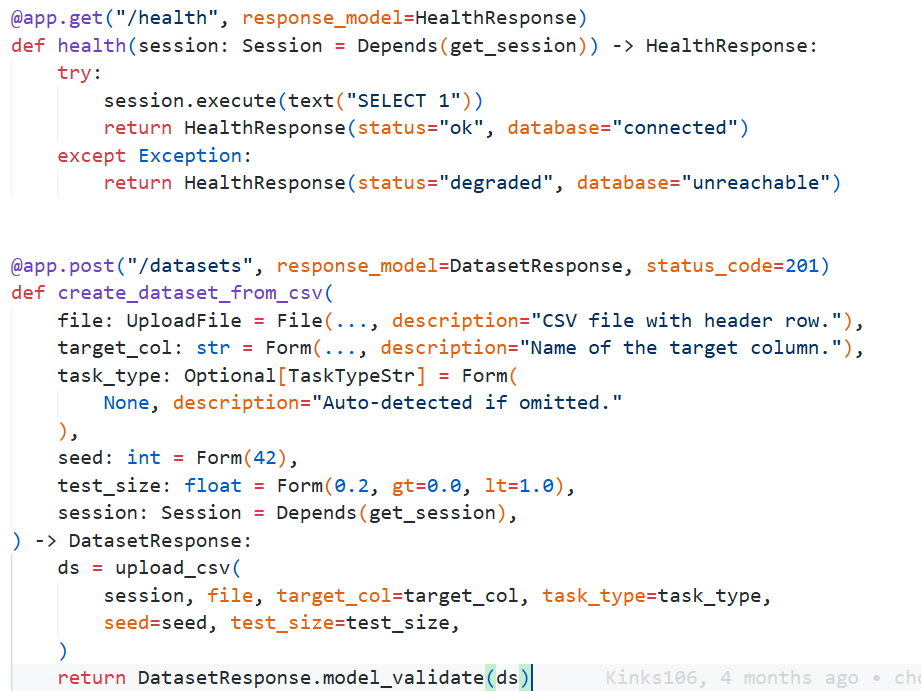
\includegraphics[width=0.9\textwidth]{figures/project_figures/screenshots/data_generation_service_1.png}
    \caption{Data--service ingestion path (dataset registration and
    split).}
    \label{fig:data-svc}
\end{figure}

\subsection{Meta-Feature Service}

For each dataset the service computes one JSON meta--feature object
with four families --- \emph{simple} (counts, missingness,
cardinality, class balance), \emph{distributional} (skewness,
kurtosis, outlier ratio), \emph{information} (mutual information,
pairwise correlation, target entropy) and \emph{landmarking} (decision
stump, linear/NB and 1--NN reference scores) --- and caches it in the
\texttt{meta\_features} table. Column typing is handled by small,
deterministic helpers (Fig.~\ref{fig:mf-helpers}).

\begin{figure}[H]
    \centering
    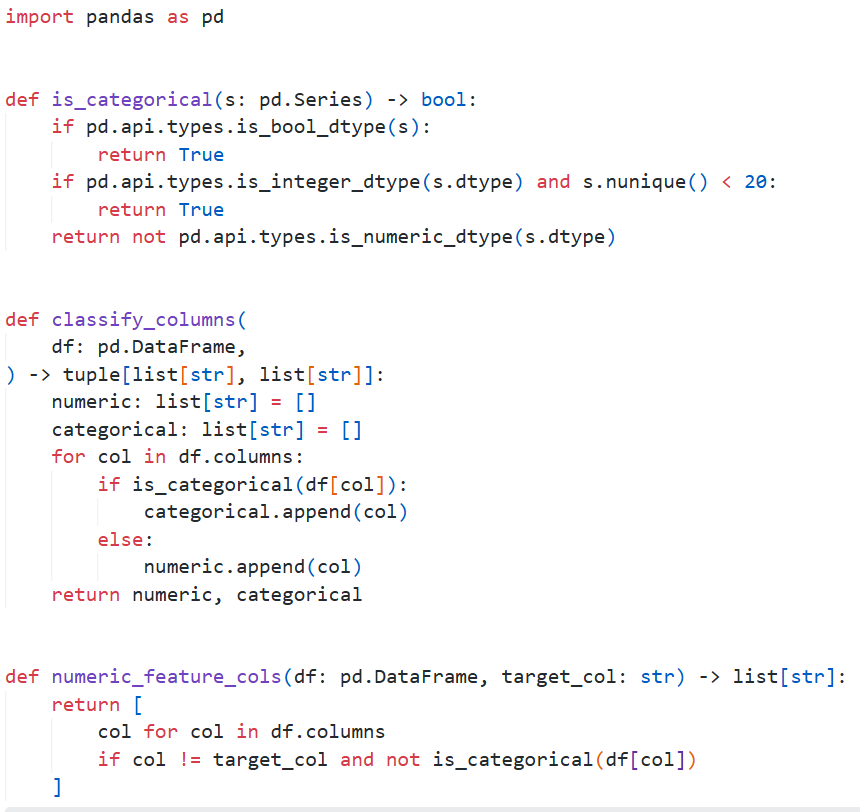
\includegraphics[width=0.78\textwidth]{figures/project_figures/screenshots/metaFetaures_helpers.png}
    \caption{Meta--feature helpers: a column is categorical if boolean,
    low--cardinality integer, or non--numeric.}
    \label{fig:mf-helpers}
\end{figure}

\subsection{Prompt Conditions: B0, B1, B2}

The three conditions are the experiment's independent variable and
differ \emph{only} in prompt content; the code that executes, scores
and persists their output is identical.

\begin{itemize}
    \item \textbf{B0 (naive).} Task description only, plus the hard
    requirement that every class/function be explicitly imported.
    \item \textbf{B1 (schema).} B0 plus a dataset--schema section:
    row/column counts, task type, target column, column dtypes and the
    first three rows.
    \item \textbf{B2 (meta--feature--guided).} B1 plus the full
    meta--feature JSON, fourteen numbered decision rules, a
    cite--your--reasoning instruction, and a \emph{mandatory,
    machine--verified} structured reasoning trace that the generated
    script must print at runtime (Fig.~\ref{fig:b2-prompt}).
\end{itemize}

\begin{figure}[H]
    \centering
    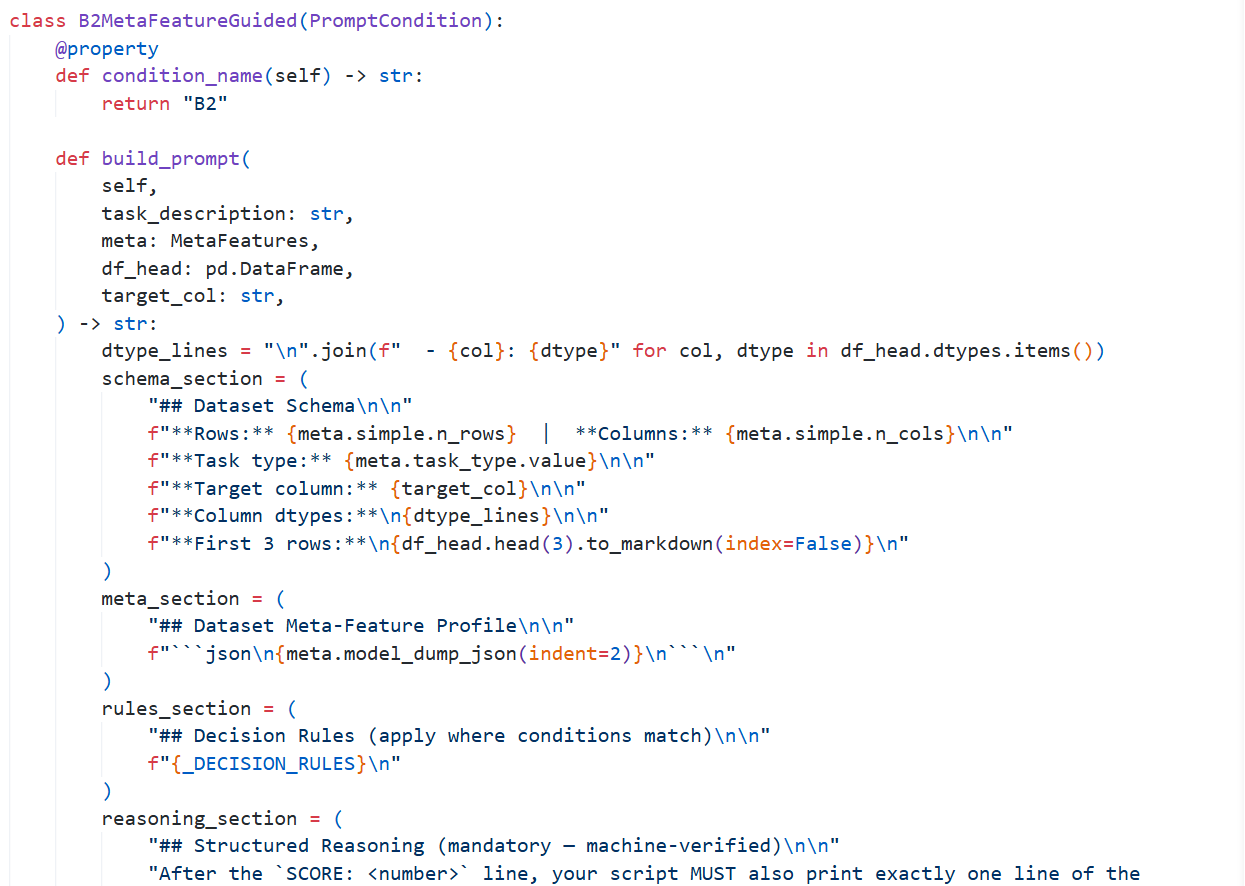
\includegraphics[width=0.95\textwidth]{figures/project_figures/screenshots/b2_metafeatures_1.png}
    \caption{The B2 prompt builder assembling the schema,
    meta--feature profile, decision rules and mandatory
    reasoning--trace sections.}
    \label{fig:b2-prompt}
\end{figure}

A consequence worth stating plainly: because the B2 reasoning trace is
printed by the \emph{generated code at runtime}, it is a post--hoc
self--report derived from the code, not a plan captured independently
\emph{before} the code. Capturing an independent pre--code plan (the
\texttt{B2R} mode of Chapter~\ref{ch:method}) is designed but not yet
wired, and is the single most important limitation of the current
verifier.

\subsection{Generation Service and RQ Worker}

The generation service records a \texttt{sweep\_jobs} row and enqueues
one Redis Queue job per cell; a worker container pulls each job, runs
\texttt{jobs.run\_cell}, and retries up to \texttt{max\_iterations}
times, feeding the classified error back to the LLM as a hint on each
retry (Fig.~\ref{fig:gen-svc}).

\begin{figure}[H]
    \centering
    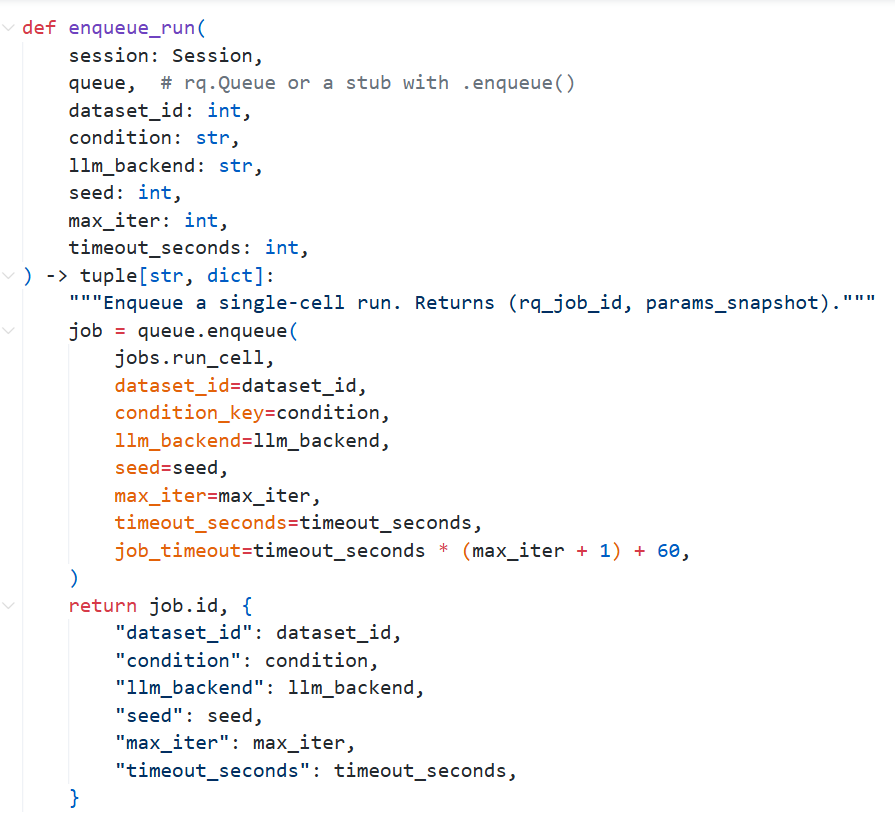
\includegraphics[width=0.82\textwidth]{figures/project_figures/screenshots/generation_service_py.png}
    \caption{Enqueuing one sweep cell as a Redis Queue job; the job
    runs \texttt{jobs.run\_cell} on a worker.}
    \label{fig:gen-svc}
\end{figure}

\subsection{Sandboxed Executor and Error Taxonomy}

Generated code is written to a temporary file and run in a fresh
Python subprocess with a per--attempt wall--clock budget; stdout,
stderr and the return code are captured and the printed
\texttt{SCORE:} line is parsed. Execution failures are classified into
the thirteen--category \texttt{ErrorCategory} taxonomy: a
priority--ordered, \texttt{stderr}--based classifier assigns the
code--failure categories (\texttt{syntax\_error}, \texttt{import\_error},
\texttt{api\_hallucination}, \texttt{shape\_mismatch},
\texttt{type\_error}, \texttt{missing\_name}, \texttt{timeout},
\texttt{resource\_limit} and others), the leakage guard assigns
\texttt{suspicious\_leakage}, and the B2 verifier assigns
\texttt{reasoning\_unfaithful}. Infrastructure--level failures (such as
a failed LLM call) are recorded under a separate \texttt{infrastructure}
label, so that LLM/prompt failures are never confused with
infrastructure failures (Fig.~\ref{fig:err-tax}).

\begin{figure}[H]
    \centering
    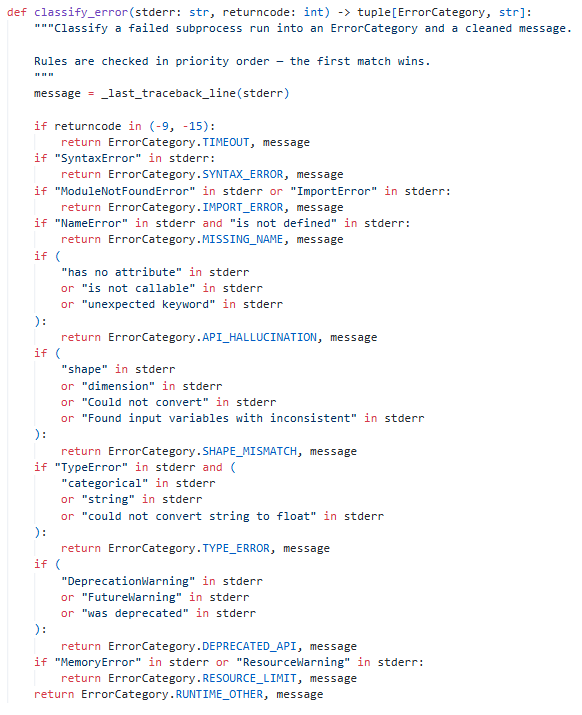
\includegraphics[width=0.66\textwidth]{figures/project_figures/screenshots/error_taxonomy.png}
    \caption{The rule--based execution--error classifier
    (\texttt{classify\_error}); the first matching rule wins.}
    \label{fig:err-tax}
\end{figure}

\subsection{Implemented Verifier (Prototype)}
\label{subsec:impl-verifier}

The implemented verifier (\texttt{execution/verification.py}) realises
a deliberately narrow subset of Chapter~\ref{ch:method}, and only for
B2 runs. For each decision in the reasoning trace it performs two
pure--Python checks:

\begin{enumerate}
    \item \textbf{Action presence.} Parse the generated code with
    \texttt{ast} into a set of referenced names (imports, called
    functions, attributes, bare identifiers). The decision passes if
    its cited \texttt{action} symbol is in that set --- catching a
    preprocessor the LLM \emph{claimed} but never used.
    \item \textbf{Value grounding.} Follow the decision's cited
    \texttt{meta\_feature} dotted path into the real meta--feature
    object and compare the LLM's cited \texttt{observed\_value} within
    a $10^{-3}$ tolerance --- catching a \emph{fabricated or
    misremembered} number.
\end{enumerate}

A run is \texttt{faithful} iff every decision passes both checks; an
unfaithful run is recorded with \texttt{error\_category =
reasoning\_unfaithful}. The current code treats an \emph{uncheckable}
value (no numeric path to compare) as not--contradicted; the proposed
three--valued verdict of Chapter~\ref{ch:method} would instead return
\textsc{unverifiable} here, and closing this gap is listed as future
work. This verifier is the mechanism behind the faithfulness result of
Chapter~\ref{ch:results} (Section~\ref{sec:rq5}).

\paragraph{RIR/PIR prototype (feature branch).} A larger prototype of
the Chapter~\ref{ch:method} verifier exists on the
\texttt{feat/rir-pir-verifier} branch (stdlib \texttt{ast} and
\texttt{dataclasses}, not merged into \texttt{main} and not wired into
the run tier). It lowers a plan into the RIR and the generated code
into an AST--based PIR, applies existence, parameter, column and
ordering rules to produce a three--valued per--claim verdict, and
aggregates these --- with criticality gating --- into a four--valued
pipeline verdict, exposed through a small command--line tool. It
realises the core of the proposed design short of the graph--based PIR
and the set--valued mapper, and has so far been exercised only on a
small set of hand--checked cases, not on the 270--run sweep.

\subsection{Persistence and Analysis}

Each cell is persisted as a \texttt{run\_results} row; the B2
\texttt{reasoning\_trace} and \texttt{verification\_report} are stored
as JSON columns and also written as \texttt{.trace.json} /
\texttt{.verification.json} sidecars to MinIO. The analysis service
exposes one read--only endpoint per research question plus
\texttt{/analysis/traces} and \texttt{/analysis/rule-usage}; because
it only reads persisted rows, every table in Chapter~\ref{ch:results}
can be regenerated without re--calling any LLM.

\section{Proposed Components (Designed, Not Yet Implemented)}

Beyond the \texttt{main} verifier, the prototype of
Section~\ref{subsec:impl-verifier} (branch
\texttt{feat/rir-pir-verifier}) already implements an AST--based
Program IR, existence / parameter / ordering / column checks,
three--valued per--claim and four--valued pipeline verdicts over a
partial taxonomy, and a standalone CLI; it is not merged into
\texttt{main}, not wired into the run tier, and not validated at the
scale of the 270--run study. The remaining parts of
Chapter~\ref{ch:method} are \emph{not} built anywhere and are not drawn
upon by the 270--run study of Chapter~\ref{ch:results}: the
graph--based (multigraph) Program IR; the set--valued
claim--to--witness mapper with learned ranking; the full mismatch
taxonomy as emitted categories; and a verification--result dashboard.
The independent pre--code reasoning capture (\texttt{B2R}) is likewise
designed but not wired.

\section{Algorithm: Implemented vs Proposed}

The implemented \texttt{main} verifier is the compact routine on the
left (presence and value grounding only); the routine on the right is
the proposed full verifier, most of which --- the RIR, the AST--based
PIR, the three--valued conjunction over presence, parameters and
ordering, and the aggregation --- is realised by the prototype of
Section~\ref{subsec:impl-verifier}, short of the graph PIR and the
set--valued mapper.

\begin{lstlisting}[language=Python,caption={Implemented: boolean faithfulness check (prototype v1).}]
def verify_reasoning(trace, code, meta):
    code_names = names_in_code(code)      # ast walk -> set[str]
    verdicts = []
    for d in trace.decisions:
        present = d.action in code_names          # presence
        value_ok = value_matches(d.observed_value,
                                 lookup(meta, d.meta_feature))  # grounding
        verdicts.append((present, value_ok))
    faithful = len(verdicts) > 0 and all(
        p and (v is not False) for p, v in verdicts)
    return VerificationReport(faithful=faithful, verdicts=verdicts)
\end{lstlisting}

\begin{lstlisting}[language=Python,caption={Proposed: full RIR--PIR claim verdicts (designed, Chapter~\ref{ch:method}).}]
def verify(plan, code):                   # PROPOSED
    rir = build_rir(plan)                  # atomic typed claims
    pir = build_pir(code)                  # attributed multigraph
    verdicts = []
    for r in rir:
        cands = mapper(r, pir)             # set-valued witness
        v = three_valued_and(presence(r, cands), semantics(r, cands),
                              parameters(r, cands), ordering(r, pir),
                              dependency(r, pir))
        verdicts.append(ClaimReport(r, cands, v, classify(r, cands, v)))
    return aggregate(verdicts)             # coverage, S_align, CMR, loc.
\end{lstlisting}

\section{Security and Privacy}

The verifier executes untrusted LLM--generated code, so the sandbox is
the main security concern. Mitigations: the subprocess runs with a
bounded wall--clock budget in a temporary working directory that is
discarded afterwards; a leakage guard flags any near--perfect score
(\texttt{>=0.995}) on a classification task for review; and raw
dataset rows are never sent to the LLM runner --- only meta--features
and column descriptors are. Static import pinning and a private--bound
API with a key are specified for deployment and are partially in place.

\section{Summary}

The implemented system is a running, seven--service FastAPI stack that
generates scikit--learn pipelines under three prompt conditions,
executes them in a sandbox, classifies failures, and --- for B2 ---
mechanically checks the reasoning trace for action presence and
value grounding, persisting everything to PostgreSQL and MinIO. The
full graph--based verifier of Chapter~\ref{ch:method} remains proposed.
The next chapter evaluates exactly what is implemented here on a real
270--cell experimental sweep.
